\documentclass{beamer}

\usepackage[UTF8,noindent]{ctexcap}
\usepackage{color}%引入颜色
\usetheme{Singapore}%使用Singapore主题
\usepackage{graphicx}%引入插图
\usepackage{ulem}%删除线
\usepackage{tikz}
\usefonttheme[onlymath]{serif}
\usepackage{minted}%[fragile]
\useoutertheme{infolines}
\usepackage[orientation=landscape,size=custom,width=16,height=9,scale=0.5,debug]{beamerposter}


\title{数学}
\author{长郡中学\ 周书予}
\date{\today}
\begin{document}\small
	
%\usebackgroundtemplate{\tikz\node[inner sep=0pt,opacity=0.3]{\includegraphics[width=14cm,height=9.6cm]{Tohsaka.png}};}
	\begin{frame}
	\titlepage
		\begin{center}
		
\includegraphics[width=2.0cm]{cj.jpg}
		$\ \ \ \ \ $
		
\includegraphics[width=2.0cm]{zsy.png}
		\end{center}
	\end{frame}
	\section{同余}
	\begin{frame}{欧几里得算法及其扩展}
		求$\gcd(a,b)$?
		\pause\\
		
		求$ax+by=\gcd(a,b)$的一组整数解?
		\pause\\
		
		由$\gcd(a,b)=\gcd(b,a \bmod b)$可得:
		
		$$ax_1+by_1=bx_2+(a-\lfloor\frac{a}{b}\rfloor b)y_2$$
		
		该不定方程的一组特解为:
		
		$$\begin{cases}
		x_1=y_2\\
		y_1=x_2-\lfloor\frac{a}{b}\rfloor y_2
		\end{cases}$$
		
		递归到$b=0$时存在一组特解$\begin{cases}x=1\\y=0\end{cases}$。
	\end{frame}
	\begin{frame}{费马小定理}
		若$p$为质数,则$a^{p-1} \equiv 1 \mod p$。
		\\
		
		常使用$a^{p-2}\equiv a^{-1} \mod p$来求逆元。
	\end{frame}
	\begin{frame}{欧拉定理及其扩展}
		若$\gcd(a,n)=1$,则$a^{\varphi(n)} \equiv 1 \mod n$。
		\\
		
		可以发现费马小定理是欧拉定理在$n$为质数时的特殊情况。
		\\
		
		若$\gcd(a,n)\neq 1$,则
		
		$$a^b\equiv\begin{cases}
		a^b &b < \varphi(n)\\
		a^{b \bmod \varphi(n)+\varphi(n)} &b \ge \varphi(n)
		\end{cases}
		\mod n$$
		
	\end{frame}
	\begin{frame}{线性求逆元}
		在$O(n)$时间内求出$1...n$在模$p$意义下的逆元。
		
		$$\begin{aligned}
		i\times \lfloor\frac{p}{i}\rfloor + (p \bmod i) &\equiv 0 &\mod p\\
		i\times \lfloor\frac{p}{i}\rfloor &\equiv -(p \bmod i) &\mod p\\
		i^{-1} &\equiv -\lfloor\frac{p}{i}\rfloor \times (p \bmod i)^{-1} &\mod p 
		\end{aligned}$$
		
		这种求法同样适用于$p$不为质数的情况。
		\\
		
		当然也可以使用$O(n+\log p)$的方法,但要注意去除与$p$不互质(不存在逆元)的数。
	\end{frame}
	\begin{frame}{}
		假设$p_1,p_2,...,p_k$两两互质,并记$P=\prod_{i=1}^kp_i$,则同余方程组
		
		$$\begin{cases}
		x \equiv a_1 \mod p_1\\
		x \equiv a_2 \mod p_2\\
		...\\
		x \equiv a_k \mod p_k
		\end{cases}$$
		
		的最小整数解为$\sum_{i=1}^ke_iw_ia_i \mod P$,其中$w_i=\frac{P}{p_i}, e_iw_i \equiv 1 \mod p_i$。
	\end{frame}
	\section{质数分解}
	\begin{frame}{唯一分解定理}
		任意正整数都可以被唯一分解成若干质数的乘积。
		
		$$n = \prod_{i=1}^k p_i^{\alpha_i}$$
		
		接下来会默认存在上述定义。
		
	\end{frame}
	\begin{frame}{干货}
		本页给出一张$n$以内最多不同质因子个数与最多约数个数的表格,在计算复杂度时,大可不必用$O(\log n)$和$O(\sqrt n)$去估计此二者。
		
		\begin{center}
			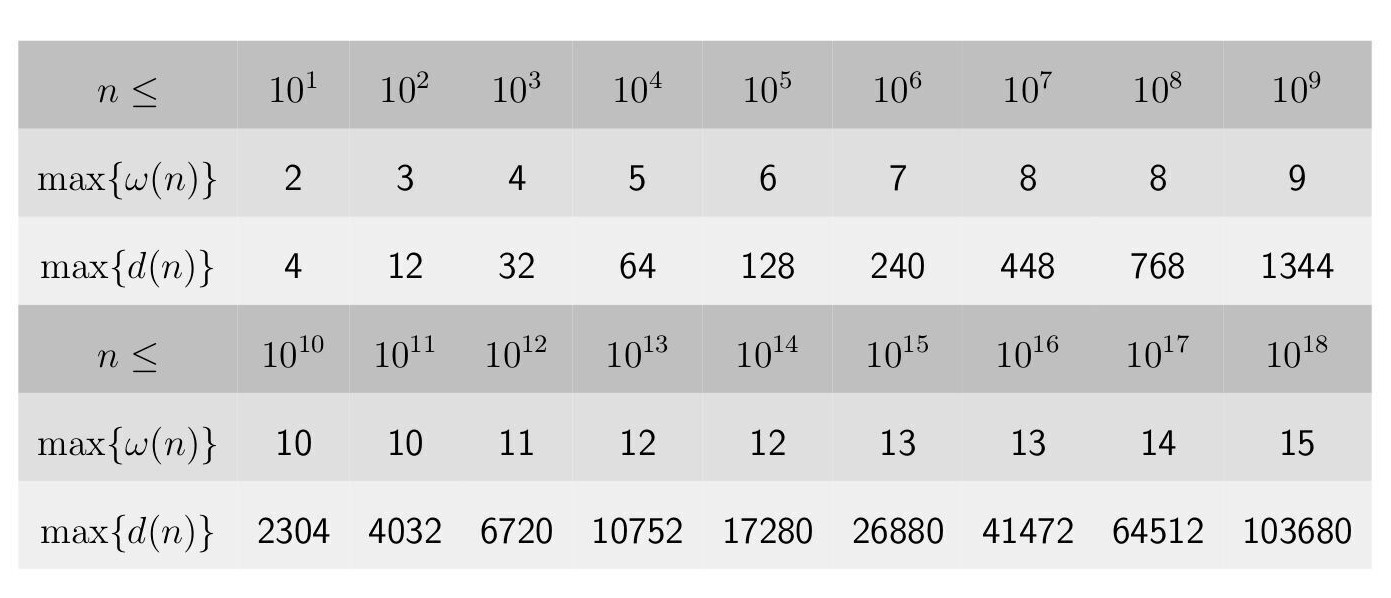
\includegraphics[width=12.0cm]{biao.jpg}
		\end{center}
	\end{frame}
	\begin{frame}{质数分解算法}
		\begin{block}{$O(\sqrt n)$分解}
			由于$n$只包含至多$1$个大于$\sqrt n$的质因子,所以可以枚举所有小于等于$\sqrt n$的质因子试除,剩下的数若大于$1$则说明也是$n$的一个质因子。
		\end{block}
		\begin{block}{$O(n)-O(\log n)$分解}
			考虑到质因子个数是$O(\log n)$级别的,因此先$O(n)$预处理$1...n$所有数的最小质因子$d_i$,每次分解时通过不断地$x \to \frac{x}{d_x}$即可实现单次$O(\log n)$分解。
		\end{block}
		\begin{block}{Pollard-Rho 质因数分解}
			复杂度$O(n^{\frac 14})$,有兴趣的同学可以去自行了解。\sout{说白了就是懒得讲}
		\end{block}
	\end{frame}
	\section{积性函数与筛法}
	\begin{frame}{积性函数}
		若$f(n)$的定义域为正整数集,值域为复数集,则称$f(n)$为数论函数。
		\\
		
		若$f(n)$为数论函数,且$f(1)=1$,对于任意互质的正整数$p,q$均满足$f(p \times q) = f(p) \times f(q)$,则称$f(n)$为积性函数。
		\\
		
		若$f(n)$为积性函数,且对于任意正整数$p,q$均满足$f(p \times q) = f(p) \times f(q)$,则称$f(n)$为完全积性函数。
	\end{frame}
	\begin{frame}{常见积性函数}
		莫比乌斯函数$\mu(n)=\prod_{i=1}^k-[\alpha_i=1]$。
		\\
		
		欧拉函数$\varphi(n)=\sum_{i=1}^n[\gcd(i,n)=1]=\prod_{i=1}^k(p_i-1)p_i^{\alpha_i-1}$。
		\\
		
		除数函数$\sigma_x(n)=\sum_{d|n}d^x=\prod_{i=1}^k\sum_{j=0}^{\alpha_i}p_i^{xj}=\prod_{i=1}^k\frac{1-p_i^{x(\alpha_i+1)}}{1-p_i^x}$。
		\\
		
		单位元函数$e(n)=[n=1]$。
		\\
		
		恒等函数$I(n)=1$。
		\\
		
		幂函数$id_x(n)=n^x$。
	\end{frame}
	\begin{frame}{Dirichlet卷积}
		数论函数$f(n)$与$g(n)$的Dirichlet卷积为$(f*g)(n)=\sum_{d|n}f(d)g(\frac nd)$,当$f$和$g$均为积性函数时,$f * g$也是积性函数。
		\\

		Dirichlet卷积满足交换律、结合律,对加法满足分配率,存在单位元函数$e(n)=[n=1]$使得$f*e=e*f=f$,且任意$f(1)\neq 0$的数论函数$f(n)$存在唯一的逆元$f^{-1}(n)$使得$f*f^{-1}=e$。
	\end{frame}
	\begin{frame}{常见Dirichlet卷积}
		\pause
		大家都知道
		
		$$\sum_{d|n}\mu(d)=[n=1],\sum_{d|n}\varphi(d)=n$$
		\pause
		
		写成Dirichlet卷积的形式就是
		
		$$\mu * I = e, \varphi * I = id_1$$
		\pause
		
		那么就很显然可以看出
		
		$$\mu * id_1 = \varphi$$
		\pause
		
		也即
		
		$$\sum_{d|n}d\mu(\frac{n}{d})=\varphi(n)$$
	\end{frame}
	\begin{frame}{筛法}
		\begin{block}{埃氏筛法}
			枚举每个质数并筛去其倍数,时间复杂度$O(n\log\log n)$。
		\end{block}
		\begin{block}{欧拉筛法(线性筛)}
			枚举每个数$n$,从小到大枚举质数$p \le p_1$并把$n\times p$筛掉,这样可以保证所有数只会被其最小质因子筛掉一次。
		\end{block}
	\end{frame}
	\section{离散对数}
	\begin{frame}{原根}
		假设$g$是质数$p$的一个原根,则$g^0,g^1,...,g^{p-2}$在模$p$意义下两两不同。
		\\
		
		也即,对于$\forall x\in[1,p-1]$,均存在$k\in[0,p-2]$使$x \equiv g^k \mod p$。
		\\
		
		由这种方式可以把模意义下的乘法转化成原根指数上的加法,也就是实现了模意义下的离散对数。
		
	\end{frame}
	\begin{frame}{大步小步算法}
		给出$a,b,p$,求$a^x \equiv b \mod p$。
		\pause\\
		
		分块,令$k=\lceil\sqrt p\rceil$,设$x=ky-z$,则有$a^{ky}=b\times a^z$。
		
		显然$y,z \in [0,k]$,因此预处理出所有$a^{ky}$并哈希存储,再枚举$z$判断是否存在相等的即可。
		\pause\\
		
		这个做法要求$\gcd(a,p)=1$,因为推导过程中用到了$a$在模$p$意义下的逆元。
	\end{frame}
	\section{组合数}
	\begin{frame}{组合数}
		$\binom{n}{m}$表示从$n$个元素中选出$m$个的方案数。\\
		
		通项:$\binom{n}{m}=\binom{n}{n-m}=\frac{n!}{m!(n-m)!}$\\
		
		递推式:$\binom{n}{m}=\binom{n-1}{m}+\binom{n-1}{m-1}$\\
		
		同行递推:$\binom{n}{m}=\binom{n}{m-1}\times\frac{n-m+1}{m}$\\
		
		二项式定理:$(x+y)^n=\sum_{i=0}^n\binom{n}{i}x^iy^{n-i}$
	\end{frame}
	\begin{frame}{格路问题}
		网格图上每步可以向右或向上走一步,从$(0,0)$走到$(n,m)$的方案数?\pause\\
		
		$\binom{n+m}{n}$,即从共计$n+m$步中选出$n$步向右走。\pause\\
		
		从$(0,0)$走到$(n,m)$,要求不碰到直线$y=x+b(n+b<m)$的方案数?\pause\\
		
		$\binom{n+m}{n}-\binom{n+m}{n+b}$,因为所有碰到直线$y=x+b$的方案均可唯一对应到一种从$(-b,b)$出发走到$(n,m)$的方案。
	\end{frame}
	\begin{frame}{Lucas定理}
		已知$p$为质数,则有$\binom{n}{m} \bmod p = \binom{\lfloor n/p \rfloor}{\lfloor m/p \rfloor}\times \binom{n\bmod p}{m \bmod p} \bmod p$。
		\pause\\
		
		另一种表述是,令$n=\overline{n_1n_2...n_k}_{(p)},m=\overline{m_1m_2...m_k}_{(p)}$(即$n,m$的$p$进制表示),则有
		
		$$\binom{n}{m} \bmod p = \prod_{i=1}^k\binom{n_i}{m_i} \bmod p$$
		
		定义$n < m$时$\binom{n}{m}=0$。
		\pause\\
		
		证明可以考虑$\binom{n}{m}$的生成函数解释是$[x^m](1+x)^n$,把此处的$n, m$按$p$进制拆分后再运用一些组合小技巧($(1+x)^p \equiv 1+x^p \mod p$)即可完成证明。
	\end{frame}
	\section{容斥原理}
	\begin{frame}{容斥原理}
		$$|\overline{\cup_{i=1}^nA_i}|=\sum_{k=0}^n(-1)^k\sum_{1 \le i_1 < i_2<...<i_k \le n}|A_{i_1}\cap A_{i_2}\cap ... \cap A_{i_k}|$$
		
		说人话就是,$n$件坏事都不发生的概率,可以通过$2^n$个子集中的坏事同时发生的概率通过加加减减得到。
	\end{frame}
	\begin{frame}{错排问题}
		有$n$个人编号为$1,...,n$,问这$n$个人站成一排全都站错位置的方案数。
		\pause\\
		
		设$f(n)$表示$n$个人随便站的方案数,显然$f(n)=n!$,设$g(n)$表示$n$个人都站错的方案数,枚举有多少个人站错了位置,我们有
		
		$$f(n)=\sum_{k=0}^n\binom{n}{k}g(k)$$
		
		然而我们是不知道$g$而知道$f$吧!
		\pause\\
		
		这里给出一个组合恒等式,接下来我们将会使用它来证明二项式反演。
		
		$$\sum_{k=0}^n(-1)^k\binom{n}{k}=[n=0]$$
		
		
	\end{frame}
	\begin{frame}{请开始你的表演}
		\pause
		首先说一句废话
		$$g(n)=\sum_{m=0}^n[n-m=0]\binom{n}{m}g(m)$$
		\pause
		然后将我们之前的那个式子代入
		$$g(n)=\sum_{m=0}^n\sum_{k=0}^{n-m}(-1)^k\binom{n-m}{k}\binom{n}{m}g(m)$$
		\pause
		利用组合恒等式进行变换(提示:考虑组合意义)
		$$g(n)=\sum_{m=0}^n\sum_{k=0}^{n-m}(-1)^k\binom{n}{k}\binom{n-k}{m}g(m)$$
		\pause
		交换求和号
		$$g(n)=\sum_{k=0}^n(-1)^k\binom{n}{k}\sum_{m=0}^{n-k}\binom{n-k}{m}g(m)$$
	\end{frame}
	\begin{frame}{证完了}
		$$g(n)=\sum_{k=0}^n(-1)^k\binom{n}{k}\sum_{m=0}^{n-k}\binom{n-k}{m}g(m)$$
		\pause
		后面的那坨就是$f(n-k)$,也就是说
		
		$$\begin{cases}
		f(n)=\sum_{k=0}^n\binom{n}{k}g(k)\\
		g(n)=\sum_{k=0}^n(-1)^{n-k}\binom{n}{k}f(k)
		\end{cases}$$
		
		此即为二项式反演。
		
	\end{frame}
	\begin{frame}{莫比乌斯反演}
		莫比乌斯反演的一般形式为
		
		$$\begin{cases}
		f(n)=\sum_{d|n}g(d)\\
		g(n)=\sum_{d|n}\mu(d)f(\frac{n}{d})
		\end{cases}$$
		
		莫比乌斯函数满足$\sum_{d|n}\mu(d)=[n=1]$。
		\pause\\
		
		\sout{证明留作课后练习。}
		\pause\\
		
		(考虑$\mu*I=e$,由$f=g*I$得$g=f*\mu$就直接证完了)
	\end{frame}
	\begin{frame}{感性理解莫比乌斯反演}
		对于一个正整数$n=\prod_{i=1}^kp_i^{\alpha_i}$,我们将其视作一个$k$维空间上的点$(\alpha_1,\alpha_2,...,\alpha_k)$。\pause\\
		
		之前提到的$g(n)$相当于是$(\alpha_1,\alpha_2,...,\alpha_k)$这个点的点权,而$f(n)$呢?\pause\\
		
		是$(\alpha_1,\alpha_2,...,\alpha_k)$这个点的$k$维前缀和,即所有满足$\beta_i \le \alpha_i$的$(\beta_1,\beta_2,...,\beta_k)$点权之和。\pause\\
		
		回顾二维前缀和、二维差分的做法,或者脑补一下三维的情况,处理$k$维前缀和时应该需要找到$2^k$个前缀和来加加减减。\pause\\
		
		然而$g(n)=\sum_{d|n}\mu(d)f(\frac nd)$哪里来的$2^k$?\pause\\
		
		冷静分析,上式枚举的所有$\mu(d)$中恰有$2^k$个非零,这揭示了莫比乌斯反演的本质是以质因子为维度的高维前缀和/差分变换。
	\end{frame}
	\section{高维前缀和}
	\begin{frame}{高维前缀和}
		用于解决高维空间中的部分和问题。由于高维空间目前还没什么实际应用,因此这种高维问题往往是由某些其他问题抽象而来,比如约数(把每个质因子的指数看做一维的坐标),子集(每一维大小为$2$的高维空间)等问题。
		
	\end{frame}
	\begin{frame}{经典问题}
		\begin{block}{description}
			给出$\{a_0,a_1,...,a_{2^n-1}\}$,求$\{b_0,b_1,...,b_{2^n-1}\}$满足
			
			$$b_i=\sum_{j \subseteq i} a_j$$
			
		\end{block}
		\begin{block}{constriction}
			$1 \le n \le 20.$
		\end{block}
		\pause
		\begin{block}{solution}
			设$f_{i,j}$表示前$i$维(这里是前$i$个二进制位)小于等于$j$(的对应二进制位),后$n-i$维等于$j$的所有$a_i$之和,初始$f_{0,j}=a_j$,转移为$f_{i,j}=f_{i-1,j}+f_{i,j-2^i}[2^i \subseteq j]$,最终答案就是$b_i=f_{n,i}$。
		\end{block}
	\end{frame}
	\section{线性代数初步}
	\begin{frame}{矩阵}
		一个$n\times m$的矩阵大概长这样:
		
		$$A=\begin{bmatrix}
		a_{1,1} & a_{1,2} & \cdots & a_{1,m}\\
		a_{2,1} & a_{2,2} & \cdots & a_{2,m}\\
		\vdots  & \vdots  & \ddots & \vdots \\
		a_{n,1} & a_{n,2} & \cdots & a_{n,m}
		\end{bmatrix}$$
		
		特别地,$n \times 1$的矩阵常被称作列向量,$1 \times m$的矩阵常被称作行向量,$1 \times 1$的矩阵有时会与矩阵元素不作区分。
	\end{frame}
	\begin{frame}{矩阵乘法}
		一个$n \times m$的矩阵$A$与一个$m \times r$的矩阵$B$的乘积定义为一个$n \times r$的矩阵$C$,其中
		
		$$c_{i,j}=\sum_{k=1}^ma_{i,k}\times b_{k,j}$$
		
		即矩阵$A$的第$i$行与矩阵$B$的第$j$列点乘的结果。\\
		
		矩阵乘法满足结合律不满足交换率。\\
		
		$n \times n$的矩阵乘法存在单位矩阵$E$满足$e_{i,j}=[i=j]$,不是所有的矩阵都存在逆矩阵。
	\end{frame}
	\begin{frame}{经典问题}
		\begin{block}{description}
			给一张$n$个点的有向图$G$,求点$1$到点$n$经过$k$条边的最短路。
		\end{block}
		\begin{block}{constriction}
			$1 \le n \le 100, 1 \le k \le 10^9.$
		\end{block}
		\pause
		\begin{block}{solution}
			$\langle+,\times \rangle$可以定义矩阵乘法,$\langle\min,+\rangle$也可以。
			
			即,定义$(A \otimes B)_{i,j}=\min_k\{a_{i,k}+b_{k,j}\}$,那么求出$G^k_{1,n}$就是答案了。
		\end{block}
	\end{frame}
	\begin{frame}{经典问题}
		\begin{block}{description}
			给一张$n$个点的有向图$G$,求点$1$到点$n$长度至少为$k$的路径经过的最少边数。
		\end{block}
		\begin{block}{constriction}
			$1 \le n \le 100, 1 \le k \le 10^9.$
		\end{block}
		\pause
		\begin{block}{solution}
			用$\langle\max,+\rangle$定义矩阵乘法。
			
			直接二分边数再套用前面做法,复杂度$O(n^3\log^2k)$。
			
			依次尝试$G^{2^{30}},G^{2^{29}}...$,复杂度$O(n^3\log k)$。
		\end{block}
	\end{frame}
	\begin{frame}{线性递推}
		矩阵乘法可以用于表示线性递推,比如最经典的斐波那契递推:
		
		$$f_k=f_{k-1}+f_{k-2}(k \ge 2)$$
		
		$$\begin{bmatrix}f_0 & f_1\end{bmatrix}\begin{bmatrix}0 & 1\\1 & 1\end{bmatrix}=\begin{bmatrix}f_1 & f_2\end{bmatrix}$$
		
		$$\begin{bmatrix}f_0 & f_1\end{bmatrix}\begin{bmatrix}0 & 1\\1 & 1\end{bmatrix}^n=\begin{bmatrix}f_n & f_{n+1}\end{bmatrix}$$
		
		这样可以把求一个$m$阶递推数列的第$n$项这个问题做到$O(m^3\log n)$的时间复杂度。
	\end{frame}
	\begin{frame}{hdu4471 Homework}
		\begin{block}{description}
			已知数列$f$的前$m$项值和另外$q$个值$f_{x_i}=y_i$,其余值满足递推式$f_k=\sum_{i=1}^mc_i\times f_{k-i}$。求$f_n$的值。
		\end{block}
		\begin{block}{constriction}
			$1 \le n \le 10^9, 1 \le m, q \le 100.$
		\end{block}
		\pause
		\begin{block}{solution}
			原做法分$q$段做,每段复杂度$O(m^3\log n)$,总复杂度$O(qm^3\log n)$。
			
			行向量乘矩阵的复杂度是$O(m^2)$的,设$A$是线性递推用到的转移矩阵,预处理出$A^1,A^2,A^4,..,A^{2^k}$再依次乘上行向量,时间复杂度$O(m^3\log n+qm^2\log n)$。
			
			可以把这里的$2$进制扩展到$B$进制,复杂度为$O(m^3B\log_Bn+qm^2\log_Bn)$。
		\end{block}
	\end{frame}
	\begin{frame}{高斯消元}
		解线性方程组
		
		$$\begin{cases}
		a_{1,1}x_1+a_{1,2}x_2+...+a_{1,n}x_n=b_1\\
		a_{2,1}x_1+a_{2,2}x_2+...+a_{2,n}x_n=b_2\\
		...\\
		a_{m,1}x_1+a_{m,2}x_2+...+a_{m,n}x_n=b_m\\
		\end{cases}$$
		
		解方程的过程可以概括为以下三步:
		
		\begin{itemize}
			\item 选取一个未被选过的未知数作为主元,选取一个未被选过的主元系数不为$0$的方程;
			\item 将这个方程中主元系数化为$1$;
			\item 通过加减消元,使其他方程中主元的系数都变成$0$。
		\end{itemize}
		
		该算法的时间复杂度为$O(n^3)$。需要注意可能存在无解或多解的情况。

	\end{frame}
	\begin{frame}{感性理解线性基}
		狭义的线性基指异或空间中的一组线性无关的基底,该空间下的任意一个向量均可以用这些基底线性表示。\pause\\
		
		实际上将数域从$\{0,1\}$扩展到$\mathbb{C}$时,线性无关的那套理论仍然成立。\\
		
		因而在解线性方程组时,可以把每个方程看做一个$n$维带权向量。\pause\\
		
		方程组无解,当且仅当存在一组线性相关的向量,经过某种线性组合后(权值同乘对应系数)得到零向量,而该零向量的权值非零。\\
		
		否则,若最大的线性无关组大小小于$n$,方程组有多解。\\
		
		否则,方程组有唯一解。
	\end{frame}
	\section{概率与期望}
	\begin{frame}{概率与期望}
		
		求概率往往可以转化为求方案数。(所以归根结底还是考数数)
		\\
		
		期望的线性性是指和的期望等于期望的和,即使拆成的两部分是相关的。
		\pause\\
		
		举个例子。假设
\includegraphics[width=0.4cm]{o_ji.jpg}和
\includegraphics[width=0.4cm]{o_mao.png}同时做一道题,
\includegraphics[width=0.4cm]{o_ji.jpg}有$p_1$的概率自己做出来,
\includegraphics[width=0.4cm]{o_mao.png}有$p_2$的概率自己做出来,
\includegraphics[width=0.4cm]{o_ji.jpg}做出来后有$q_1$的概率告诉
\includegraphics[width=0.4cm]{o_mao.png}怎么做,
\includegraphics[width=0.4cm]{o_mao.png}做出来后有$q_2$的概率告诉
\includegraphics[width=0.4cm]{o_ji.jpg}怎么做。求
\includegraphics[width=0.4cm]{o_ji.jpg}和
\includegraphics[width=0.4cm]{o_mao.png}做出的总题数的期望。
		\pause\\
		
		尽管
\includegraphics[width=0.4cm]{o_ji.jpg}和
\includegraphics[width=0.4cm]{o_mao.png}是否做出这道题这件事是相关的,但单独考虑每个人,
\includegraphics[width=0.4cm]{o_ji.jpg}做出这题的概率是$p_1+(1-p_1)p_2q_2$,
\includegraphics[width=0.4cm]{o_mao.png}做出这题的概率是$p_2+(1-p_2)p_1q_1$,因此总题数的期望就是这两者之和。
	\end{frame}
	\section{数学例题选讲}
	\subsection{apio2019 奇怪装置}
	\begin{frame}{apio2019 奇怪装置}
		\begin{block}{description}
			有一个奇怪的装置,在$t$时刻会显示数对$((t+\lfloor\frac tB\rfloor) \bmod A, t \bmod B)$。给出$n$个不交的连续时间段$[l_i,r_i]$,问这个装置在这些时间段内会显示出多少种不同的数对。
		\end{block}
		\begin{block}{constriction}
			$1 \le n \le 10^6, 1 \le A, B \le 10^{18}, 0 \le l_i \le r_i \le 10^{18}.$
		\end{block}
		\pause
		\begin{block}{solution}
			可以发现存在循环节$\frac{AB}{\gcd(A,B+1)}$。
			
			因此所有区间对循环节取模,问题变成在$[0,\frac{AB}{\gcd(A,B+1)})$上的覆盖问题,差分统计即可。
		\end{block}
	\end{frame}
	\subsection{snoi2019 数论}
	\begin{frame}{snoi2019 数论}
		\begin{block}{description}
			给出正整数$P,Q,T$,大小为$n$的整数集$A$和大小为$m$的整数集$B$,求:
			
			$$\sum_{i=0}^{T-1}[i \bmod P \in A][i \bmod Q \in B]$$
			
			换言之,就是求有多少小于$T$的非负整数$x$满足$x$除以$P$的余数属于$A$且$x$除以$Q$的余数属于$B$。
		\end{block}
		\begin{block}{constriction}
			$1 \le n, m, P, Q \le 10^6, 1 \le T \le 10^{18}.$
		\end{block}
		\pause
		\begin{block}{solution}
			$x\to (x+P) \bmod Q$会形成$\gcd(P,Q)$个长度为$\frac{Q}{\gcd(P,Q)}$的环。
		
			枚举$x\bmod P$的值(即枚举$a_i$),问题变成求有多少$0\le x\le \lfloor\frac{T-1-a_i}{P}\rfloor$满足$(Px+a_i)\bmod Q\in B$。其实就是求从$a_i$出发走$\lfloor\frac{T-1-a_i}{P}\rfloor$步能到达的所有点的点权和。根据环长讨论一下即可,复杂度$O(P+Q)$。
		\end{block}
	\end{frame}
	\subsection{jxoi2018 游戏}
	\begin{frame}{jxoi2018 游戏}
		\begin{block}{description}
			初始时有$r-l+1$个数$l,l+1,...,r$,每次操作为随机选取一个数并删除其所有倍数,求删完所有数的期望操作次数模$10^9+7$。
		\end{block}
		\begin{block}{constriction}
			$1 \le l \le r \le 10^7.$
		\end{block}
		\pause
		\begin{block}{solution}
			根据倍数关系建拓扑图,删完整张图当且仅当删除了所有入度为零的点。
			
			求入度为零的点的个数即求有多少个数除去最小质因子后$< l$。
			
			假设入度为零的点有$m$个,设$n=r-l+1$,枚举操作次数,答案为$\frac{1}{n!}\sum_{i=m}^{n}i\times m \times \binom{n-m}{i-m}(i-1)!(n-i)!$。
		\end{block}
	\end{frame}
	\subsection{51nod1769 Clarke and math 2}
	\begin{frame}{51nod1769 Clarke and math 2}
		\begin{block}{description}
			已知数论函数$f(n),g(n)$满足
			
			$$g(i)=\sum_{i_1|i}\sum_{i_2|i_1}...\sum_{i_k|i_{k-1}}f(i_k)$$
			
			给出$f(1)...f(n)$,求$g(1)...g(n)$对$10^9+7$取模后的结果。
		\end{block}
		\begin{block}{constriction}
			$1 \le n \le 10^5, 1 \le k \le 10^{10^5}, 0 \le f(i) < 10^9+7.$
		\end{block}
		\pause
		\begin{block}{solution}
			写成Dirichlet卷积的形式是$g=f*I^k$。
			
			考虑$I^k(n)$怎么求。这是一个积性函数,因此只需要考虑$I^k(p^{\alpha})$怎么求即可。这等价于长度为$k$值域为$[0,\alpha]$的单调不降序列方案数,等价于把$\alpha$个球放入$k$个盒子里的方案数,即$\binom{\alpha+k-1}{\alpha}$。
		\end{block}
	\end{frame}
	\subsection{snoi2017 遗失的答案}
	\begin{frame}{snoi2017 遗失的答案}
		\begin{block}{description}
			求从$\{1,2,...,n\}$中选出一个非空子集,其最大公约数恰好为$G$,最小公倍数恰好为$L$的方案数。
			
			此外有$q$次询问,每次询问给出一个正整数$a_i$,询问选出的非空子集必须包含$a_i$时的方案数。
			
			输出答案对$10^9+7$取模后的结果。
		\end{block}
		\begin{block}{constriction}
			$1 \le n, G, L \le 10^8, q \le 10^5, 1 \le a_i \le n.$
		\end{block}
		\pause
		\begin{block}{solution}
			分别考虑每个质因子,$G$和$L$限制了所有数在这个质因子的幂次,即位于区间$[l,r]$之间,且至少一个取到$l$,至少一个取到$r$。而$10^8$内最多只有$8$个不同质因子,对每个质因子是否取到上下界状压,那么$[1,n]$内每个合法的数都可以用一个长度不超过$16$的二进制状态表示,问题转化为求从合法的数中选出一个子集按位或为全集的方案数,\href{https://files.cnblogs.com/files/zhoushuyu/sol.pdf}{\color{pink}{可以参考这里的题解}}。
		\end{block}
	\end{frame}
	\subsection{bzoj4767 两双手}
	\begin{frame}{bzoj4767 两双手}
		\begin{block}{description}
			有一张无限大的棋盘以及两种移动方式$(x_1,y_1)$和$(x_2,y_2)$,同时棋盘上存在$k$个障碍点不能经过。求从$(0,0)$走到$(n,m)$不经过障碍点的方案数模$10^9+7$。
		\end{block}
		\begin{block}{constriction}
			$0 \le |x_1|, |y_1|, |x_2|, |y_2|, k, n, m \le 1000, (x_1,y_1)\times (x_2,y_2) \neq 0.$
		\end{block}
		\pause
		\begin{block}{solution}
			可以通过解方程把$(x_1,y_1),(x_2,y_2)$转化成$(1,0),(0,1)$,从而转化成常规的格路问题。
			
			设$f_i$表示从$(0,0)$出发不经过任何其他障碍点到达第$i$个障碍点的方案数,转移时容斥,枚举经过的第一个障碍点$j$,从$j$走到$i$的方案数是组合数。时间复杂度$O(k^2)$。
		\end{block}
	\end{frame}
	\subsection{hncpc2019H 有向图}
	\begin{frame}{hncpc2019H 有向图}
		\begin{block}{description}
			一张$n+m$个点的图,初始在$1$号点,每次在$i$号点时有$P_{i,j}$的概率走到$j$号点,保证$\forall i\in[n+1,n+m],P_{i,j}=[i=j]$。可以发现经过无限次行走后停留在前$n$号点上的概率是$0$,求停留在后$m$号点每个点的概率模$10^9+7$。
		\end{block}
		\begin{block}{constriction}
			$1 \le n+m \le 500, \forall i\in[1,i], 0 < P_{i,j} < 1$且$\sum_{j=1}^{n+m}P_{i,j}=1.$
		\end{block}
		\pause
		\begin{block}{solution}
			设$f_i(i\in[1,n])$表示$i$号点的期望经过次数,则可列出方程:
			
			$$\begin{cases}
			f_i=\sum_{j=1}^nf_jP_{j,i}+1&i=1\\
			f_i=\sum_{j=1}^nf_jP_{j,i}  &i>1
			\end{cases}$$
			
			解出$f_i$后,易得$ans_j=\sum_{i=1}^nf_iP_{i,j}$。
		\end{block}
		
	\end{frame}
	\subsection{tjoi2019 唱、跳、rap和篮球}
	\begin{frame}{tjoi2019 唱、跳、rap和
\includegraphics[width=0.7cm]{o_xzz.jpg}}
		\begin{block}{description}
			最喜欢唱、跳、rap和
\includegraphics[width=0.4cm]{o_xzz.jpg}的同学数量分别为$a,b,c,d$。
\includegraphics[width=0.4cm]{o_ji.jpg}和
\includegraphics[width=0.4cm]{o_mao.png}想选出$n$个同学排成一队,但是他们不希望队伍中有连续四个人依次最喜欢唱、跳、rap和
\includegraphics[width=0.4cm]{o_xzz.jpg},因为这样他们就会聚在一起讨论
\includegraphics[width=0.4cm]{o_cxk.png}。求排队的方案数模$998244353$,两种方案不同当且仅当存在某个位置上的同学的喜好不同。
		\end{block}
		\begin{block}{constriction}
			$1 \le n,a,b,c,d \le 5000, a+b+c+d \ge n.$
		\end{block}
		\pause
		\begin{block}{solution}
			强制枚举$i$组同学讨论
\includegraphics[width=0.4cm]{o_cxk.png},剩下的位置随便填,容斥计算答案。记$f_i$表示从$\{a-i,b-i,c-i,d-i\}$个学生中选出$n-4i$个排队的方案数,答案即为$\sum_{i\ge 0}(-1)^i\binom{n-3i}{i}f_i$。
			
			单次计算$f_i$显然可以$O(n^2)$dp,但$i$从小到大枚举时dp数组的变化不大,因此可以考虑维护前两者的dp数组和后两者的dp数组,从而把时间复杂度做到单次$O(n)$。总时间复杂度$O(n^2)$。
		\end{block}
	\end{frame}
	\subsection{codeforces1097D Makoto and a Blackboard}
	\begin{frame}{codeforces1097D Makoto and a Blackboard}
		\begin{block}{description}
			有一个数$n$,每次操作为随机选择$n$的一个约数$m$并将$n$替换成$m$,求$k$次操作后$n$的期望值模$10^9+7$。
		\end{block}
		\begin{block}{constriction}
			$1 \le n \le 10^{15}, 1 \le k \le 10^4.$
		\end{block}
		\pause
		\begin{block}{solution}
			根据乘法分配律,只需要对每个$p_i^{\alpha_i}$求出答案即可。
			
			只需要考虑指数。问题转化成给一个数$\alpha_i$,每次把当前的数$x$等概率随机变成$[0,x]$的一个整数,求$k$次操作后剩下的数是$[0,\alpha_i]$的概率。
			
			直接$O(\alpha_i^2k)$暴力dp或者$O(\alpha_i^3\log k)$矩乘。
		\end{block}
	\end{frame}
	\subsection{codeforces1097F Alex and a TV Show}
	\begin{frame}{codeforces1097F Alex and a TV Show}
		\begin{block}{description}
			你需要编写一种数据结构来维护$n$个可重集合,支持四种操作:
			\begin{itemize}
				\item 将$S_x$设为$\{v\}$
				\item 将$S_x$设为$S_y + S_z$,操作后$|S_x|=|S_y|+|S_z|$
				\item 将$S_x$设为$S_y\times S_z$,这里的$A \times B$定义为$\{\gcd(a,b)|a\in A, b\in B\}$,操作后$|S_x|=|S_y|\times|S_z|$
				\item 询问$S_x$中$v$元素的数量
			\end{itemize}
			
			由于一些原因,你只需要输出每个询问的答案对$2$取模后的结果。
		\end{block}
		\begin{block}{constriction}
			$1\le n, m \le 10^5, 1 \le v \le 7000.$
		\end{block}
	\end{frame}
	\begin{frame}{codeforces1097F Alex and a TV Show}
		\begin{block}{solution}
			对每个可重集维护一个数组$a_i$表示可重集中有多少个数是$i$的约数,可以发现这样的$a$数组可以唯一的表示一个可重集。
			
			第二种操作本质是$a$数组对应位相加,第三种操作本质是$a$数组对应位相乘,这个结论读者自证不难。
			
			由于只需要输出$\bmod 2$意义下的答案,所以可以用一个\texttt{bitset<7000>}来维护$a$数组,这样对应位相加变成了按位异或,对应位相乘变成了按位与。
			
			维护$a$数组后,对于一次询问$v$,答案为$\sum_{v|u}a_u\mu(\frac{u}{v})$,由于$-1 \equiv 1 \bmod 2$,所以只需要再维护$7000$个\texttt{bitset<7000>}表示询问$v$时哪些位的莫比乌斯函数不为零就好了。
			
			时间复杂度为$O(\frac{7000m}{\omega})$。
		\end{block}
	\end{frame}
	
	\section{The end}
	\begin{frame}{}
		\begin{center}
			{\Huge 谢谢大家!}
			
			\vspace{5 ex}
			
			感谢
\includegraphics[width=0.4cm]{o_ji.jpg},
\includegraphics[width=0.4cm]{o_mao.png}、
\includegraphics[width=0.4cm]{o_xzz.jpg}以及
\includegraphics[width=0.4cm]{o_cxk.png}的友情出镜。
		\end{center}
		
		
	\end{frame}
\end{document}